\section{Resolução Questão 12}

\begin{frame}[fragile]{Enunciado da Questão}
    Considere a função densidade de probabilidade (fdp) abaixo:
\[
f(x) =
\begin{cases}
3e^{-3x}, & x \geq 0 \\
0, & \text{caso contrário}
\end{cases}
\]

\begin{enumerate}
    \item[(a)] Calcule a função de distribuição acumulada (FDA) e sua inversa.
    \item[(b)] Gere uma amostra de 10.000 observações usando o método da FDA inversa.
    \item[(c)] Esboce a fdp teórica e o histograma da amostra. Eles são semelhantes?
    \item[(d)] Calcule a média e a variância populacional.
    \item[(e)] Calcule a média e a variância amostral.
\end{enumerate}
\end{frame}

% --- RESOLUÇÃO ITEM (a) ---
\begin{frame}{Item (a): Cálculo da FDA}
Dada a fdp da distribuição exponencial com $\lambda = 3$:
\[
f(x) = 3e^{-3x} \quad \text{para } x \geq 0
\]
A função de distribuição acumulada (FDA), $F(x)$, é a integral da fdp:
\[
F(x) = \int_{0}^{x} 3e^{-3t} \, dt
\]
Resolvendo a integral, temos:
\[
\int_{0}^{x} 3e^{-3t} \, dt = \left[ -e^{-3t} \right]_{0}^{x} = -e^{-3x} - (-e^0) = 1 - e^{-3x}
\]
Portanto, a FDA é:
\[
F(x) =
\begin{cases}
1 - e^{-3x}, & x \geq 0 \\
0, & x < 0
\end{cases}
\]
\end{frame}

\begin{frame}{Item (a): Inversa da FDA}
Para encontrar a função inversa da FDA, $F^{-1}(u)$, fazemos $u = F(x)$ e isolamos $x$.
\[
u = 1 - e^{-3x}
\]
\[
e^{-3x} = 1 - u
\]
\[
\ln(e^{-3x}) = \ln(1 - u)
\]
\[
-3x = \ln(1 - u)
\]
\[
x = -\frac{1}{3} \ln(1 - u)
\]
A função inversa da FDA, para $0 < u < 1$, é:
\[
F^{-1}(u) = -\frac{\ln(1 - u)}{3}
\]
\end{frame}

% --- RESOLUÇÃO ITEM (b) ---
\begin{frame}[fragile]{Item (b): Geração da Amostra (Scilab)}
\begin{lstlisting}
// Parâmetros
lambda = 3;
n = 10000;

// FDA inversa da exponencial
function x = exponencial_inv(u, lambda)
    x = -log(1 - u) / lambda;
endfunction

// 1. Gerar n observações de uma distribuição Uniforme(0,1)
U = rand(n, 1);

// 2. Aplicar a FDA inversa para obter a amostra exponencial
amostra_fda = exponencial_inv(U, lambda);

// Exibindo a média da amostra para verificação
printf("Média amostral: %.4f\n", mean(amostra_fda));
// Valor teórico esperado: 1/3 = 0.3333
\end{lstlisting}
\end{frame}

\begin{frame}{Visualização da Amostra Gerada}
\frametitle{Item (b): Histograma da Amostra}
\begin{figure}
    \centering
    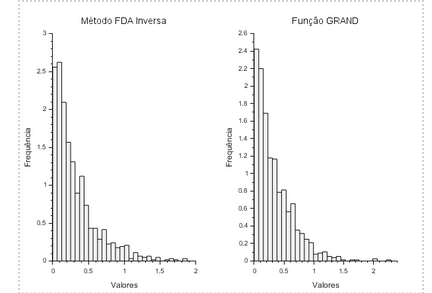
\includegraphics[width=0.6\textwidth]{figures/FDA_inversa_GRAnd.png}
    \caption{Histograma da amostra de 10.000 observações gerada com o método da FDA inversa.}
    \label{fig:hist_fda}
\end{figure}
\end{frame}

% --- RESOLUÇÃO ITEM (c) ---
\begin{frame}[fragile]{Item (c): Código da Comparação (Scilab)}
\begin{lstlisting}
// Vetor de pontos para a PDF teórica
x_teorico = linspace(0, max(amostra_fda), 200);
pdf_teorica = lambda * exp(-lambda * x_teorico);

// Plotar histograma normalizado e PDF teórica
scf();
histplot(30, amostra_fda, normalization=%t); // Normalizado
plot(x_teorico, pdf_teorica, 'r-', 'LineWidth', 2);

// Configurações do gráfico
title('Comparação: PDF Teórica vs Histograma da Amostra');
xlabel('Valores');
ylabel('Densidade de Probabilidade');
legend(['Histograma (n=10000)'; 'PDF Teórica (λ=3)']);
\end{lstlisting}
\end{frame}

\begin{frame}{Item (c): Comparação Gráfica}
\frametitle{Comparação: PDF Teórica vs Histograma}
\begin{figure}
    \centering
    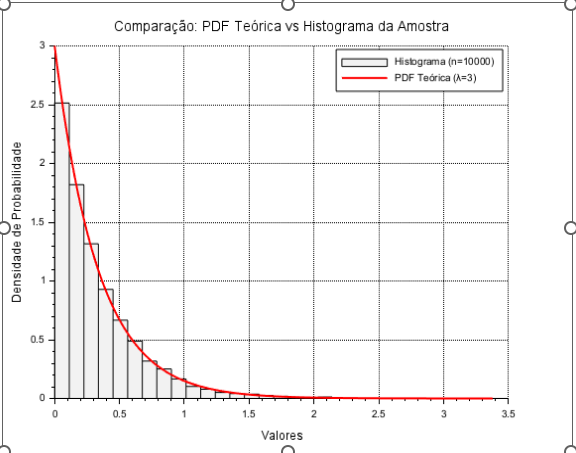
\includegraphics[width=0.7\textwidth]{figures/comparacao.png}
    \caption{O histograma da amostra se aproxima muito bem da curva da fdp teórica, validando o método de geração.}
    \label{fig:comparacao}
\end{figure}
\end{frame}


% --- RESOLUÇÃO ITEM (d) ---
\begin{frame}{Item (d): Média e Variância Populacional}
A \textbf{média} (ou esperança) $\mathbb{E}(X)$ de uma exponencial com parâmetro $\lambda$ é:
\[
\mathbb{E}(X) = \frac{1}{\lambda}
\]
Com $\lambda = 3$, temos:
\[
\mathbb{E}(X) = \boxed{\frac{1}{3}}
\]
\vspace{1cm}
A \textbf{variância} $\text{Var}(X)$ de uma exponencial com parâmetro $\lambda$ é:
\[
\text{Var}(X) = \frac{1}{\lambda^2}
\]
Com $\lambda = 3$, temos:
\[
\text{Var}(X) = \frac{1}{3^2} = \boxed{\frac{1}{9}}
\]
\end{frame}

% --- RESOLUÇÃO ITEM (e) ---
\begin{frame}[fragile]{Item (e): Média e Variância Amostral}
Usando o Scilab para calcular as estatísticas da amostra gerada:
\begin{lstlisting}
// 'amostra_fda' é o vetor com 10.000 observações

media_amostral = mean(amostra_fda);
variancia_amostral = variance(amostra_fda);

printf("Média Teórica: %.4f\n", 1/3);
printf("Média Amostral: %.4f\n\n", media_amostral);

printf("Variância Teórica: %.4f\n", 1/9);
printf("Variância Amostral: %.4f\n", variancia_amostral);
\end{lstlisting}
\vspace{0.5cm}
\textbf{Resultado esperado:} Os valores da média e variância amostral devem ser muito próximos dos valores teóricos ($1/3 \approx 0.3333$ e $1/9 \approx 0.1111$).
\end{frame}